\documentclass{beamer}
\usepackage[utf8]{inputenc}
\usepackage[T1]{fontenc}
\usepackage{ngerman}
\usepackage{amsmath,amssymb}
\usepackage{pgfplots}
\pgfplotsset{compat=1.18}

\begin{document}

\begin{frame}
    \frametitle{Die Exponentialverteilung}
{\small

    \textbf{Definition:} Zufallsvariable $X$ mit Parameter $\lambda>0$  
\[
    X \sim \mathrm{Exp}(\lambda)
    \quad\Longleftrightarrow\quad
    f_X(x) = 
        \begin{cases}
            \lambda\,e^{-\lambda x}, & x\ge0,\\
            0, & x<0.
        \end{cases}
\]

\smallskip
  \textbf{Normierung:}
\[
    \int_{0}^{\infty} f_X(x)\,\mathrm{d}x
    = \int_{0}^{\infty} \lambda e^{-\lambda x}\,\mathrm{d}x
    = \lambda\bigl[-\tfrac{1}{\lambda}e^{-\lambda x}\bigr]_{0}^{\infty}
    = 1.
\]

\smallskip
\textbf{Verteilungsfunktion:}
\[
    F_X(x) = P(X\le x)
    = \int_{0}^{x} \lambda e^{-\lambda t}\,\mathrm{d}t
    = 1 - e^{-\lambda x},
    \quad \lim_{x\to\infty}F_X(x)=1.
    \]
}
  \bigskip
  \begin{center}
    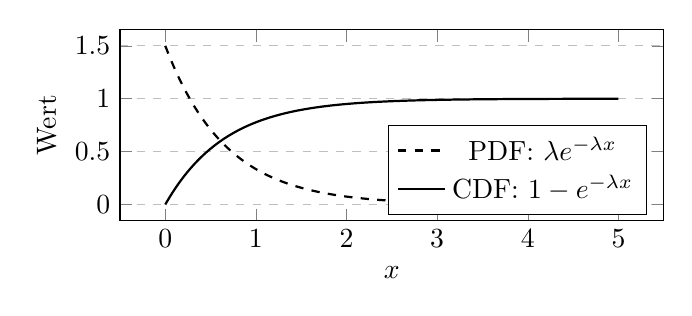
\begin{tikzpicture}
      \begin{axis}[
        width=0.7\textwidth,
        height=4cm,
        domain=0:5,
        samples=200,
        xlabel=$x$,
        ylabel={Wert},
        legend pos=south east,
        ymajorgrids=true,
        grid style=dashed,
      ]
        \addplot[thick, dashed] {1.5*exp(-1.5*x)}; 
        \addlegendentry{PDF: $\lambda e^{-\lambda x}$}

        \addplot[thick] {1-exp(-1.5*x)};
        \addlegendentry{CDF: $1 - e^{-\lambda x}$}
      \end{axis}
    \end{tikzpicture}
  \end{center}
\end{frame}

\begin{frame}
  \frametitle{Erwartungswert der Exponentialverteilung}

  Für \(X\sim\mathrm{Exp}(\lambda)\) gilt
  \[
    E[X]
    = \int_{0}^{\infty} x\,\lambda e^{-\lambda x}\,\mathrm{d}x
    = \int_{0}^{\infty}
      \underbrace{x}_{u}
      \;\underbrace{\lambda e^{-\lambda x}}_{dv}
      \,\mathrm{d}x.
  \]

  Mit partieller Integration (\(u=x,\;dv=\lambda e^{-\lambda x}dx\)) folgt
  \[
    u = x,\quad
    dv = \lambda e^{-\lambda x}\,dx,
    \quad
    du = \,dx,\quad
    v = -e^{-\lambda x}.
  \]
  Daher
  \[
    \int_{0}^{\infty} x\,\lambda e^{-\lambda x}\,dx
    = \Bigl[\,\underbrace{x}_{u}\,\underbrace{(-e^{-\lambda x})}_{v}\Bigr]_{0}^{\infty}
      - \int_{0}^{\infty}
        \underbrace{1}_{du}
        \,\underbrace{(-e^{-\lambda x})}_{v}
      \,dx
    = 0 + \int_{0}^{\infty} e^{-\lambda x}\,dx
    = \Bigl[-\tfrac{1}{\lambda}e^{-\lambda x}\Bigr]_{0}^{\infty}
    = \frac{1}{\lambda}.
  \]

  \vfill
  \[
    \boxed{E[X] = \frac{1}{\lambda}.}
  \]
\end{frame}

\begin{frame}
  \frametitle{Erwartungswert der Exponentialverteilung}

  Für \(X\sim\mathrm{Exp}(\lambda)\) gilt
  \[
    E[X]
    = \int_{0}^{\infty} x\,f_X(x)\,\mathrm{d}x
    = \int_{0}^{\infty} x\,\lambda e^{-\lambda x}\,\mathrm{d}x.
  \]

  \medskip
  Mit partieller Integration (\(u=x,\;dv=\lambda e^{-\lambda x}dx\)) setzt man
  \[
    u = x,\quad dv = \lambda e^{-\lambda x}\,dx,
    \qquad
    du = dx,\quad v = -e^{-\lambda x}.
  \]
  Dann
  \[
    \int_{0}^{\infty} x\,\lambda e^{-\lambda x}\,dx
    = \Bigl[x\,(-e^{-\lambda x})\Bigr]_{0}^{\infty}
      - \int_{0}^{\infty} 1\cdot(-e^{-\lambda x})\,dx
    = 0 + \int_{0}^{\infty} e^{-\lambda x}\,dx
    = \left[-\tfrac{1}{\lambda}e^{-\lambda x}\right]_{0}^{\infty}
    = \frac{1}{\lambda}.
  \]

  \vfill
  \[
    \boxed{E[X] = \frac{1}{\lambda}.}
  \]
\end{frame}


\begin{frame}
  \frametitle{Zentraler Grenzwertsatz für Summen und Mittelwert}

  \[
    S_n \;=\;\sum_{i=1}^n X_i
    \quad\Longrightarrow\quad
    S_n \;\overset{\mathrm{d}}{\approx}\;
    \mathcal{N}\bigl(n\, \mu,\; \sqrt{n} \cdot \sigma \bigr)
  \]

  \[
    \bar X_n \;=\;\frac{1}{n}\sum_{i=1}^n X_i
    \;=\;\frac{1}{n}S_n
    \quad\Longrightarrow\quad
    \bar X_n \;\overset{\mathrm{d}}{\approx}\;
    \mathcal{N}\bigl(\mu,\; \tfrac{\sigma}{\sqrt{n}} \bigr)
  \]
\end{frame}


\end{document}